%%%%%%%%%%%%%%%%%%%%%%%%%%%%%%%%%%%%%%%%%
% Short Sectioned Assignment
% LaTeX Template
% Version 1.0 (5/5/12)
%
% This template has been downloaded from:
% http://www.LaTeXTemplates.com
%
% Original author:
% Frits Wenneker (http://www.howtotex.com)
%
% License:
% CC BY-NC-SA 3.0 (http://creativecommons.org/licenses/by-nc-sa/3.0/)
%
%%%%%%%%%%%%%%%%%%%%%%%%%%%%%%%%%%%%%%%%

%----------------------------------------------------------------------------------------
%	PACKAGES AND OTHER DOCUMENT CONFIGURATIONS
%----------------------------------------------------------------------------------------

\documentclass[paper=a4, fontsize=12pt, xcolor=dvipsnames]{scrartcl} % A4 paper and 11pt font size

\usepackage[T1]{fontenc} % Use 8-bit encoding that has 256 glyphs
\usepackage{fourier} % Use the Adobe Utopia font for the document - comment this line to return to the LaTeX default
\usepackage{amsmath,amsfonts,amsthm} % Math packages
\usepackage{natbib}
\usepackage{pgfplots}
\usepackage{wrapfig}
\usepackage{sidecap}

%\usepackage{minted}

% Bibliographie auf deutsch
%\usepackage{harvard}
%\renewcommand{\harvardand}{und} 

\usepackage{xcolor}
\usepackage[utf8]{inputenc} 
%\usepackage[ngerman]{babel}

\usepackage{latexsym}
\usepackage{textcomp}
\usepackage[T1]{fontenc}
\usepackage{bm}% bold math
\usepackage{hyperref}
\usepackage{graphicx}
\usepackage{caption}
\usepackage{subcaption}
\usepackage{verbatim}
\usepackage{epsfig}
\usepackage{framed,color}
\usepackage[usenames,dvipsnames]{pstricks}
\usepackage{epsfig}
\usepackage{tikz}
\usepackage{lipsum} % Used for inserting dummy 'Lorem ipsum' text into the template
\usepackage{sectsty} % Allows customizing section commands
\allsectionsfont{\centering \normalfont\scshape} % Make all sections centered, the default font and small caps

\usepackage{fancyhdr} % Custom headers and footers
\pagestyle{plain} % Makes all pages in the document conform to the custom headers and footers
\fancyhead{} % No page header - if you want one, create it in the same way as the footers below
\fancyfoot[L]{} % Empty left footer
\fancyfoot[C]{} % Empty center footer
\fancyfoot[R]{\thepage} % Page numbering for right footer
%\renewcommand{\headrulewidth}{0pt} % Remove header underlines
%\renewcommand{\footrulewidth}{0pt} % Remove footer underlines
\setlength{\headheight}{13.6pt} % Customize the height of the header
\usepackage{eso-pic}
\numberwithin{equation}{section} % Number equations within sections (i.e. 1.1, 1.2, 2.1, 2.2 instead of 1, 2, 3, 4)
\numberwithin{figure}{section} % Number figures within sections (i.e. 1.1, 1.2, 2.1, 2.2 instead of 1, 2, 3, 4)
\numberwithin{table}{section} % Number tables within sections (i.e. 1.1, 1.2, 2.1, 2.2 instead of 1, 2, 3, 4)

\setlength\parindent{0pt} % Removes all indentation from paragraphs - comment this line for an assignment with lots of text
\setcapindent{1cm} 

%----------------------------------------------------------------------------------------
%	TITLE SECTION
%----------------------------------------------------------------------------------------

\newcommand{\horrule}[1]{\rule{\linewidth}{#1}} % Create horizontal rule command with 1 argument of height

\title{ 
\normalfont \normalsize 
\textsc{Albert-Ludwigs-University Freiburg} \\ [25pt] % Your university, school and/or department name(s)
\horrule{0.5pt} \\[0.4cm] % Thin top horizontal rule
\huge $J_2$-Molecule \\ % The assignment title
\horrule{2pt} \\[0.5cm] % Thick bottom horizontal rule
}

\author{Friedrich Schüßler and Volker Karle} % Your name

\date{\normalsize\today} % Today's date or a custom date

\begin{document}
\maketitle

\newpage
\tableofcontents
\thispagestyle{empty}
\newpage
\setcounter{page}{1}


%----------------------------------------------------------------------------------------
%	PROBLEM 1
%----------------------------------------------------------------------------------------


\section{Introduction}
\subsection{Overview}
In the following experiment, we will analyse the spectral band of absorbtion of the iodine 2 molecule 
with spectroscopal methods. For the given conditions, the expected observation stems almost 
entirely from one electronic transition, the 
\begin{equation}
    B ^3\Pi_{\sigma \, \mathrm{u}}^{+} \quad <- \quad X ^1\Sigma_{\sigma \, \mathrm{u}}^{+}
\end{equation}
transition. Since iodine is a relativly heavy di-atomic molecule, it has vibrational modes that 
split up the total energy of the molecule considerably and are visible in the spectrum with the 
resolution of the given spectrometer. The energy is further changed by rotational modes of the 
atoms, which however don't show up as separate lines but rather widen the observed bands, as the 
resolution is not high enough. 
The observed data is then used to calculated characteristical constants for the molecule, such as 
the dissipation energy $D_e$ and the mean radius $r_c$. 

\subsection{Historic review}
The structure of molecular iodine ($I_2$) has been studied various times in physical chemistry 
during the last century. One of the first thorough measurements of the spectral bands was done in 
1923 by the German physicist Reinhard Meck \cite{mecke1923bandenspektrum}. The vibrational states 
were correctly numbered for the first time by Loomis \cite{loomis1927correlation}, who analysed 
the fluorecence spectrum earlier measured by Wood \cite{wood1911} for $v = 26$.



\subsection{Theoretical Foundations}
When describing molecules in the framework of quantum mechanics, we are faced with the problem of 
finding solutions to the non-relativistic and time-independent Schrödinger-equation
\begin{equation}
    \hat{H} \psi = \Big[- \frac{\hbar^2}{2m} 
        \nabla^2 + \hat{V}(\mathbf{r}) \Big] \psi = E \psi
\end{equation}
where $\psi$ are eigenfunctions of the hamilton operator $\hat{H}$.
It is out of the scope of this introduction to give a complete
and comprehensive introduction into quantum mechanics, therefore
we will not only leave out the most important results, but
furthermore mention those kind of results without proof which
we need for further calculations. For the beginning it is
important to at least write down the characterisic properties
of the harmonic oscillator, in order to perturbate this
kind of potential onto a unharmonic oscillator, which will be
treated with secondorder perturbationtheory. After this we 
immedeatly come to the molecule orbitals, which we need
to resolve the energy levels being measured in this experiment.
\subsubsection{Harmonic Oscillator}
The potential for the harmonic oscillator is given as follwing:
\begin{equation}
    \hat{V}= \frac{m}{2} \omega^2 \hat{x}^2
\end{equation}
To solve this equation, the most convenient method is to
introduce different basis of operators in which it is very
convenient to write down the energy
~\cite{fliessbach2008quantenmechanik}, which we will not do here
but state the eigenvalues (with quantumnumber $\nu$)
of the energy without proof
(see also figure~\ref{fig:harmonic1}):
\begin{equation}
    H(\nu) = \left ( \nu + \frac{1}{2} \right )\hbar \omega 
    \quad \text{with $\nu\in \mathbb{N_0}$}
\end{equation}
where the wavefunctions
   are given by
   \begin{equation}
    \psi_n(x)= \left(\frac{m\omega}{\pi\hbar}
    \right)^\frac{1}{4}
\frac{1}{\sqrt{2^nn!}} H_n
\left(\sqrt{\frac{m\omega}{\hbar}} x \right)
e^{-\frac{1}{2}\frac{m\omega}{\hbar}x^2}
\end{equation}
and $H_n$ are the hermite polynomials: 
\begin{equation}
H_n(x)=(-1)^n e^{x^2}\frac{d^n}{dx^n}\left(e^{-x^2}\right) 
\end{equation}
\begin{figure}
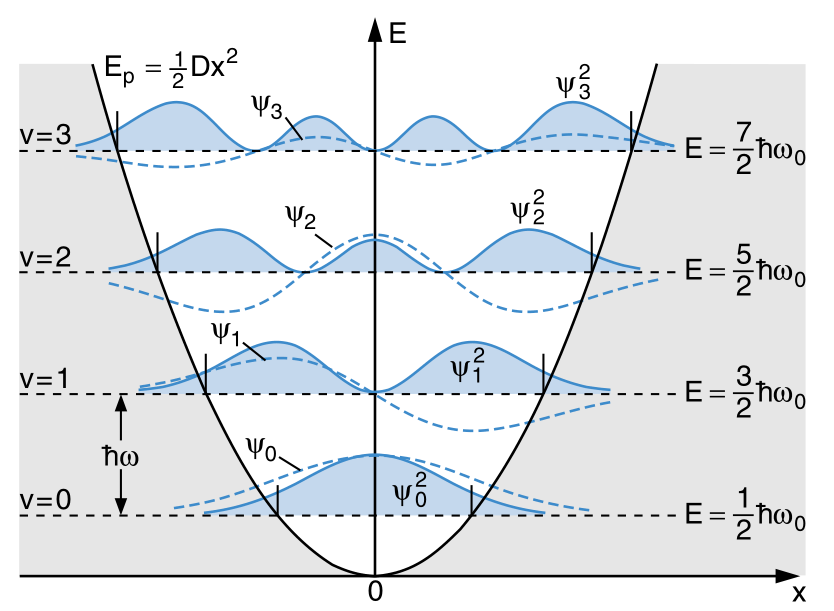
\includegraphics[width=15cm]{pics/harmonic1}
\caption{Energy levels of the harmonic oscillator with its 
    related wavefunctions\cite{Demtroeder1}.}
\label{fig:harmonic1}
\end{figure}
This potential is of outstanding importance for our experiment,
since the real potential will be aproximated in a region near
the minimum with a harmonic potential. 
To a few problems we can find the analytical solution
to the schrödingerequation, but to most
of the problems we need to approximate the solution with regards to an analyical
solution which is given. In the following sections we will introduce
the time-independent Perturbationtheory and give an example with the 
anharmonic oscillator how such an approximation can take place.
\subsubsection{Timeindependent Perturbationtheory}
We are following~\cite{fliessbach2008quantenmechanik}.
Lets assume we know the Eigenvalues and -functions of a specific
Hamiltonoperator $\hat{H_0}$ of the
unperturbed system (we further assume the eigenspaces to be
seperable, so we have no degeneracy. The case of degeneracy
can be done analogously) 
, numbered with $n\in \mathbb{N}$:

\begin{equation}
\hat{H_0} |n\rangle = \epsilon_n |n\rangle 
\end{equation}
and now we search for the solution of the perturbated Hamiltonian:
\begin{equation}
    \hat{H}|\psi \rangle = E|\psi \rangle 
\end{equation}
by means of the initial Hamiltonian:
\begin{equation}
    \hat{H} = \hat{H_0} + \lambda \hat{V}
\end{equation}
where we perturbate the original Hamiltonian with the Potential
$\hat{V}$ and give an approximate Soluation as long as Perturbation
is not of the same order of magnitude as $H_0$. 
The next step will be to apply this to the anharmonic 
Oscillator in order to get an estimation about the energyeigenvalues.
At first we have introduced a new parameter $\lambda$, which is the 
strength of the perturbation; for $\lambda = 1$ we have the problem
we want to solve, for $\lambda = 0 $ we arrive at the unperturbed
problem. Now we can expand in this parameter:
\begin{align}
    E_n(\lambda) &= \epsilon_n + \sum_{\nu =1}^{\infty} \lambda^\nu
    E_{n,\nu} \\ 
    |\psi_n(\lambda)\rangle &=
    |n\rangle + \sum_{\nu =1}^{\infty} \lambda^\nu
    |\psi_{n,\nu}(\lambda)\rangle
\end{align}
As result the solutions we are looking for will become:
\begin{align}
    E_n &= \epsilon_n + E_{n,1} + E_{n,2} + \cdots\\ 
    |\psi_n \rangle &= |n\rangle + |\psi_{n,1} \rangle + \cdots 
\end{align}
We assume for now that this series is converging and plug it into
the Schrödingerequation:
\begin{equation}
    (\hat{H_0} + \lambda \hat{V})
   \left( |n\rangle + \sum_{\nu =1}^{\infty} \lambda^\nu
        |\psi_{n,\nu}(\lambda)\rangle \right) =
\epsilon_n + \sum_{\nu =1}^{\infty} \lambda^\nu
    E_{n,\nu}  
    \left( |n\rangle + \sum_{\nu' =1}^{\infty} \lambda^{\nu'}
        |\psi_{n,\nu'}(\lambda)\rangle \right) 
\end{equation}
Now we can impose that the different powers of $\lambda$ have to
match on both sides and receive a set of equations:
\begin{align}
    \hat{H_0} |n\rangle &= \epsilon_n |n\rangle\\
    \hat{H_0} |\psi_{n,1}\rangle + \hat{V}|n\rangle &=
    \epsilon_n |\psi_{n,1}\rangle + E_{n,1}|n\rangle \label{eq:dev1}\\
    \hat{H_0} |\psi_{n,2}\rangle + \hat{V}|\psi_{n,1}\rangle &=
    \epsilon_n |\psi_{n,2}\rangle + E_{n,1}|\psi{n,1}\rangle 
    + E_{n,2}|n\rangle \label{eq:dev2}\
\end{align}
This set of equations yield recursive the Solutions of $E_{n,1}$,
$E_{n,2}$ and so on. Now we expand these single Wavefunctions 
into the new basis of energyeigenfunctions $|m \rangle$ with $m\in 
\mathbb{N}$:
\begin{equation}
    |\psi_{n,1}\rangle = \sum_{m=1}^{\infty} a_{nm} |m \rangle
    \label{eq:psi_expansion}
\end{equation}
We can plug this expansion now into into equation~\eqref{eq:dev1}:
\begin{equation}
    \sum_{m=1}^{\infty} (\epsilon_n - \epsilon_m) a_{nm} |m\rangle
    + E_{n,1} |n\rangle = \hat{V}|n \rangle
\end{equation}
With the Projection onto the dual eigenstate $\langle k|$ we can
use the orthonormality $\langle k | m \rangle = \delta_{m,k}$ 
of the energyeigenfunctions:
\begin{equation}
     (\epsilon_n - \epsilon_k) a_{nk} 
     + E_{n,1}\delta_{n,k}  = \langle k |\hat{V}|n \rangle
\end{equation}
For the case $k = n$ we get:
\begin{equation}
    E_{n,1} = \langle k |\hat{V}|n \rangle
\end{equation}
and for $k\neq m$:
\begin{equation}
    a_{n,k} = \frac{\langle k |\hat{V}|n \rangle}
    {\epsilon_n - \epsilon_k} \label{eq:a_nk}
\end{equation}
Equation~\eqref{eq:a_nk} together with~\eqref{eq:psi_expansion} 
gives us now:
\begin{equation}
    |\psi_{n}\rangle = |n\rangle + \lambda \sum_{m\neq n}^{\infty}
    \frac{\langle m |\hat{V}|n \rangle}{\epsilon_n - \epsilon_m}  
    |m \rangle + \lambda a_{n,n} + \mathcal{O}(\lambda^2)
\end{equation}
Now we can set $a_{n,n}=0$ (see footnote~\footnote{
Again we can use orthonormality:
\begin{equation*}
    1\overset{!}{=} \langle \psi_n|\psi_{n}\rangle 
    = \left | 1 + \lambda a_{nn} \right |^2 + \lambda^2
    \sum_{m\neq n}^{\infty}
    \left | \frac{\langle m |\hat{V}|n \rangle}
        {\epsilon_n - \epsilon_m} \right |^2 = 
    1 + \lambda (a_{n,n} + a^*_{n,n}) + \mathcal{O}(\lambda^2)
\end{equation*}
When $\lambda > 0 $ this results into:
\begin{equation*}
    a_{n,n} + a^*_{n,n} = 0 \Rightarrow \Re  [a_{n,n}] = 0
\end{equation*}
Since the Wavefunctions 
are invariant with respect to a phase $\phi$,
we can set without limitations $a_{nn}$ to zero.} for
further details) and we arrive
at:
\begin{equation}
    |\psi_{n}\rangle = |n\rangle + \lambda \sum_{m\neq n}^{\infty}
    \frac{\langle m |\hat{V}|n \rangle}{\epsilon_n - \epsilon_m}  
    |m \rangle  + \mathcal{O}(\lambda^2)
\end{equation}
For the Energy we can make use of the third equation and go to
the second order:
\begin{equation}
|\psi_{n,2}\rangle  = \sum_{m=1}^{X} b_{n,m} |m \rangle 
\end{equation}
We can plug this analogously into equation~\eqref{eq:dev2} and
arrive at:
\begin{equation}
 \sum_{m}^{\infty} (\epsilon_n - \epsilon_m) b_{nm} |m\rangle +
 \sum_{m}^{\infty} E_{n,1} a_{n,m} |m \rangle + E_{n,2} |n \rangle =
 \sum_{m}^{\infty} a_{n,m} \hat{V} |m \rangle
\end{equation}
Where again we use the orthonormality. For $k=n$ we get:
\begin{equation}
    E_{n,2} = \sum_{m}^{\infty} a_{n,m} \langle n |\hat{V}|m\rangle
= \sum_{m\neq n}^{\infty}\frac{|\langle n | \hat{V} | m \rangle |^2}
    {\epsilon_n - \epsilon_m}
\end{equation}
For $k\neq n$ we would arrive at the explicit formula for $b_{n,m}$
but this is not necessary for the further computations.
As final result we therefore get:
\begin{align}
    E_n &\approx \epsilon_n + \langle n|\hat{V} | n \rangle +
\sum_{m\neq n}^{\infty}\frac{|\langle n | \hat{V} | m \rangle |^2}
    {\epsilon_n - \epsilon_m} \\
    |\psi_n \rangle &\approx 
    |n\rangle + \sum_{m\neq n}^{\infty}
    \frac{\langle m |\hat{V}|n \rangle}{\epsilon_n - \epsilon_m}  
    |m \rangle 
\end{align}
\subsection{The anharmonic oscillator}
Lets assume we have solved the harmonic oscillator with 
\begin{align}
    \hat{H_0} &= \frac{\hat{p}^2}{2m} 
    + \frac{1}{2} m \omega_0^2\hat{x}^2 \\
    \hat{H_0}|n \rangle &= \epsilon_n |n \rangle \\
    \epsilon_n &= \hbar \omega_0 \left (n+ \frac{1}{2} \right)
\end{align}
Now perturbe this system with a kubic potential potential:
\begin{equation}
\hat{V} =\lambda \hat{x}^3
\end{equation}
Hence we can use the perturbation theory in linear order.
Since the parity of $\hat{V}$ is odd, the expectation value has 
to be zero:
\begin{equation}
    E_{n,1} = \lambda \langle n | \hat{x}^3 | n \rangle = 0 
\end{equation}
The wavefunctions have to be corrected as follows:
\begin{equation}
    |\psi_{n,1} \rangle = \sum_{m\neq n}^{\infty}
    \frac{\langle m |\hat{V}|n \rangle}{\epsilon_n - \epsilon_m}  
    |m \rangle 
    = \frac{\lambda}{\hbar \omega}
    |\psi_{n,1} \rangle = \sum_{m\neq n}^{\infty}
    \frac{\langle m |\hat{x}^3|n \rangle}{\epsilon_n - \epsilon_m}  
    |m \rangle 
\end{equation}
Now we have to calculate the matrix elements. Therefore we
introduce the creation- and annihilationoperator 
which are defined by $\hat{x}$:
\begin{equation}
    \hat{x} = \sqrt{\frac{\hbar}{2m\omega}}(\hat{a}^\dagger +
        \hat{a})
\end{equation} 
Now we can calculate iteratively the matrixelements
\footnote{
    Here we make use how $\hat{a}$ and $\hat{a}^\dagger$ act 
    on the eigenfunctions $|n\rangle$:
\begin{align*}
    \hat{x}|n'\rangle = \sqrt{\frac{\hbar}{2m\omega}}
    \left ( \sqrt{n' + 1}|n'+1\rangle 
        + \sqrt{n'}|n' - 1 \rangle \right ) 
\end{align*}
Applying once more:
\begin{align*}
\hat{x}^2|n'\rangle = \frac{\hbar}{2m\omega}
\left ( \sqrt{(n' + 1)(n' + 2)}|n'+2\rangle 
            + (2n' + 1) |n' \rangle
            + \sqrt{(n'(n'-1)}|n' - 2 \rangle \right ) 
\end{align*}
And applying for the third time:
\begin{align*}
    \hat{x}^3|n'\rangle &= \sqrt[3]{\left (\frac{\hbar}{2m\omega}\right )^2}
( \sqrt{(n' + 1)(n' + 2)(n'+3)}|n'+3\rangle 
    + 3 \sqrt{(n'+1)^3}|n' +1 \rangle  \\
 &+ 3 \sqrt{(n')^3}|n' -1 \rangle   
            + \sqrt{(n'(n'-1)(n'-2)}|n' - 3 \rangle  ) 
\end{align*}
Now this yields the matrixelements which we need:
\begin{align}
    \langle n | \hat{x}^3 | n' \rangle &=  
    \sqrt{\left (\frac{\hbar}{2m\omega}\right)^3}
( \sqrt{(n' + 1)(n' + 2)(n'+3)}\delta_{n,n'+3} 
    + 3 \sqrt{(n'+1)^3}\delta_{n,n'-1}  \\
    &+ 3 \sqrt{(n')^3}\delta_{n,n'-1}   
    + \sqrt{(n'(n'-1)(n'-2)}\delta_{n,n'-3}  ) 
\end{align}

}. After applying the justified indices, since only $n'=n\pm 1$ and
$m = n \pm 3 $ are not zero, we arrive at:
\begin{equation}
\begin{aligned}
    |\psi_{n,1} \rangle &= \frac{\lambda}{\hbar \omega}
    \sqrt{\left(\frac{\hbar}{2m\omega}\right)^3}
    ( -\frac{1}{3}\sqrt{(n + 1)(n + 2)(n+3)}|n+3\rangle 
    - 3 \sqrt{(n+1)^3}|n +1 \rangle  \\
 &+ 3 \sqrt{(n)^3}|n -1 \rangle  
    +\frac{1}{3} \sqrt{(n(n-1)(n-2)}|n - 3 \rangle  ) 
\end{aligned}
\end{equation}
We can also calculate the energy corrections:
\begin{equation}
    E_{n,2} = \langle n | \hat{V} | \psi_{n,1} \rangle 
    = \lambda \langle n | \hat{x}^3 | \psi_{n,1} \rangle 
\end{equation}
Which yields:
\begin{equation}
\begin{aligned}
    E_{n,2} &= \frac{\hbar^2 \lambda^2}{2 m^3 \omega ^4}
    \left[-\frac{1}{3}(n+1)(n+2)(n+3)
        -9(n+1)^3 + 9n^3 + \frac{1}{3}n(n-1)(n-2)
        \right ] \\
    &= -\frac{\hbar^2 \lambda^2}{2 m^3 \omega ^4}
    \left[ 30n^2+ 30n + 11 \right ]\\
    &= -\frac{30 \hbar^2 \lambda^2}{2 m^3 \omega ^4}
    \left[\left(n + \frac{1}{2} \right)^2 + \frac{11}{30} \right ]\\
\end{aligned}
\end{equation}
If we had a look at the closed form for all orders, we would
notice the possibility to expand the Energy Difference in terms
of powers of the original Energy $(n+\frac{1}{2})$ which we will
state here without proof:
\begin{equation}
    E_n = \hbar \omega_{0,0} \left(n + \frac{1}{2} \right) 
    - \hbar \omega_{0,1} \left(n + \frac{1}{2} \right)^2  
    + \hbar \omega_{0,2} \left(n + \frac{1}{2} \right)^3  
    + \cdots
\end{equation}
We did not include the small derivation independent of $n$,
since we will look only at energydifferences. Notice that
the final result is only valid for a small, odd Perturbation. 
\subsubsection{Energylevels and Wavefunctions
    of two-atomic molecules}

First we will write down the full Equations of the two-atomic
molecule and investigate after which parts we can further
simplify (This whole derivation will follow \cite{staatsexamen}):
\begin{equation}
        \hat{H}\psi = E\psi 
\end{equation}
Where we can expand the Hamiltonian in the position-space,
where we already split into the electrons ($i$) and the 
two nucleons $A$ and $B$:
\begin{equation}
    \hat{H} = \frac{-\hbar^2}{2} 
        \underbrace{\left(
        \sum_{i}{\frac{\nabla_i^2}{m_e}}
        +\frac{\nabla_A^2}{M_A} +\frac{\nabla_B^2}{M_B}
\right)}_{
\substack{\text{kinetic energy}\\\text{of electrons and nucleons}}}
+ \underbrace{\sum_{i>j}{\frac{e^2}{|r_i - r_j|}}
    }_{\substack{\text{potential energy}\\\text{electron-electron}}}
 - \underbrace{\sum_{i}{\frac{Z_A e^2}{|r_i - r_A|}}
 }_{\substack{\text{potential energy}\\\text{electron-nucleon $A$}}}
 - \underbrace{\sum_{i}{\frac{Z_B e^2}{|r_i - r_B|}}
 }_{\substack{\text{potential energy}\\\text{electron-nucleon $B$}}}
 +  \underbrace{\frac{Z_A Z_B e^2}{|r_A - r_B|}
 }_{\substack{\text{potential energy}\\\text{nucleon $A$ - nucleon $B$}}}
\end{equation}
Now we split the electronsolutions and the nucleonsolutions such
that the solutions of the electrons change only little when the
distance of the nucleons change, which is known as the
\textsc{BORN-OPPENHEIMER}-Approximation \cite{staatsexamen}:
\begin{align}
    \psi &= \psi_E ( \cdots r_i \cdots) \psi_N(r_A, r_B) \\
    \hat{ H}_E\psi_E &= \left(- \sum_{i}{\frac{\hbar^2\nabla_i^2}{2m_e}}
    + \sum_{i>j}{\frac{e^2}{|r_i - r_j|}}
    - \sum_{i}\frac{Z_A e^2}{|r_i - r_A|}
    - \sum_{i}\frac{Z_B e^2}{|r_i - r_B|}
    + 
    \right ) \psi_E = 
 E_E \psi_E \\
 \hat{H}_N\psi_N &= \left (
 -\frac{\hbar^2\nabla_A^2}{2M_A} -\frac{\hbar^2\nabla_B^2}{2M_B}
    - \sum_{i}\frac{Z_A e^2}{|r_i - r_A|}
    - \sum_{i}\frac{Z_B e^2}{|r_i - r_B|}
 + \frac{Z_A Z_B e^2}{|r_A - r_B|}
 \right ) \psi_N
=  E_N \psi_N 
\end{align}
Where we fixed the positions for the Hamiltonian
of the electrons such that they are not included in the
wavefunction. The interaction between electrons and the nucleons
will not be neglected since the Wavefunctions $\psi_E$ are still
dependend of the distance between the nucleons $r$. 
\par
The obvious problem arises when trying to solve these equations,
since it is not possible without great difficulties. 
The next step is to build up trialsolutions of $\psi_E$, 
consisting of solutions when there is only one electron and a
nucleon. These solutions are called one-electron orbital wave
and will be abbreviated
with \textit{MO} (\textit{Molecule orbital}) and the trialsolutions
will be built up upon linear combinations of those
(\textit{Linear combinations of atomic orbitals} method,
\textit{LCAO}). This method was first introduced 1929 by 
Sir John Lennard-Jones and has to be used with caution, since
it is only in certain limits applicable. The parameters which
appear in these combinations can be constrained by 
expectationvalues measured in experiments.
Now we will turn our attention to the movement of nucleons.
Since in our case we only have two of them, we can perform 
a coordinatetransform to the normal coordinates with a fictional
nucleon with mass
\begin{equation}
    \mu = \frac{M_A M_B}{M_A + M_B}
\end{equation}
so that our new Schrödingerequation with the wavefunction of the
fictional nucleon will look like:
\begin{equation}
    \nabla^2 \psi_N + \frac{2\mu}{\hbar^2} 
    \left[ E - V(r) \right] = 0 
\end{equation}
The Laplaceoperator written in spherical coordinates will yield
the spherical harmonics as eigenfunctions, so we can use a 
seperational ansatz for our wavefunction:
\begin{equation}
    \psi_N(r,\theta,\rho) = \frac{1}{r} S(r)Y(\theta,\rho)
\end{equation}
with the corresponding
differentialoperator, where $J\in \mathbb{N}_0$
corresponds to the Quantumnumber of the total angular momentum:
\begin{equation}
    \frac{\partial}{\sin\theta \partial \theta}\left (\sin\theta
    \frac{\partial Y}{\partial \theta}\right ) +
\frac{1}{\sin^2\theta} \frac{\partial^2 Y}{ \partial\rho^2}
 + J(J+1)Y = 0
\end{equation}
Thus we can split the rest of the wavefunction into the 
radial component of the Operator:

\begin{equation}
    \frac{d^2 S}{dr^2} + \frac{2\mu}{\hbar^2}
\left ( E - V(r) - \frac{J(J+1)\hbar^2}{2\mu r^2} \right ) S =0 
\end{equation}

If there is no further degeneracy (for instance due to not
considered interactions like spin) we can in theory write
down the Energyeigenvalues in terms of the two Quantumnumbers
$nu$ and $J$:
\begin{equation}
    E = E_{\nu,J}
\end{equation}
Practically this is not possible, so we look at two extrem cases.
\paragraph{The rigid Rotator} is based on the approximation to
fix the range of the two nuclei ($r =$const.) and so we only
look at $V(r)=0$ and $\frac{S(r)}{r} = 1$. We immedeatly get
the solution (since the sphericalharmonics already resolved
the eigenvalues):
\begin{equation}
    E = \frac{J(J+1)\hbar^2}{2\mu r^2}
\end{equation}
\paragraph{The rotationless Oscillator} just neglects the terms
arising from rotation, which is, looking at the lengthscale of
the former calculated eigenvalues, not inopportune.
The Operator then becomes:
\begin{equation}
    \frac{d^2 S}{dr^2} + \frac{2\mu}{\hbar^2}
    \left ( E - V(r) ) = 0 \right )
\end{equation}
The Eigenfunctions and -values are now very dependent on the 
potential energy $V(r)$ which is until now not a known 
potential, because it includes the repulsion due to the
pauliprinciple of the electronorbits as well as the attraction
of the charges. Furthermore the physical nature of dissociation
of the two nucleons also has to be encoded into it.
It is not possible to solve the potential analytically, but 
we will start to write down the properties already known:
\begin{itemize}
        \item Pauliprinciple:
            $\lim\limits_{r \rightarrow 0}{V(r)} = \infty $
        \item Dissociated nucleons:
$\lim\limits_{r \rightarrow \infty}{V(r)} = const. $
\item Before the Dissociation: Attraction of the nucleons with
    the maximal attraction at $r_e$ and the Dissociationenergy
    $D_e$ defined by 
    $ \lim\limits_{r \rightarrow \infty}{V(r)} - V(r_e)=: D_e$ 
\end{itemize}
The idea is now to capture this properties into the coefficients
of the taylored Potential and by doing so resolving the principle
physical behavior:
\begin{equation}
    V(r) = V(r_e) 
   + \frac{\partial V(r)}{\partial r}|_{r=r_e}(r - r_e)
   + \frac{\partial^2 V(r)}{2!\partial r^2}|_{r=r_e}(r - r_e)^2
   + \frac{\partial^3 V(r)}{3!\partial r^3}|_{r=r_e}(r - r_e)^3
   + \cdots
\end{equation}
As first approximation for energies near the minimum $r=r_e$ we
can finally use the harmonic potential. The constant term
$V(r_e)$ can be dropped since we are only interested in 
potential differences.
\begin{equation}
    V_{harm}(r) =
    \frac{\partial^2 V(r)}{2\partial r^2}|_{r=r_e}(r - r_e)^2
    =: \frac{k_e}{2}(r-r_e)^2
\end{equation}
Following this approach we can use the energyeigenvalues of the
harmonic oscillator in order to approximate
the vibrational states $\nu$:
\begin{equation}
    E_\nu =\sqrt{\frac{k_e}{\mu}}\hbar \left (\nu
        + \frac{1}{2}\right )
\end{equation}
In order to chose a more convenient unit we transform this
equation into $cm^{-1}$:
\begin{equation}
    G_{harm}(\nu) = \frac{E}{hc} = \omega_0 (\nu + \frac{1}{2})
    \quad \text{with the frequency} \quad
    \omega_0 = \frac{1}{2\pi c} \sqrt{\frac{k_e}{\mu}}
\end{equation}
The wider we leave the regime around $r_e$, speaking about 
higher vibrational states, the worse approximation with a harmonic
oscillator becomes. Qualitatively this is the case when energies
come nearer to the dissociation energy. An adhoc solution is 
to treat this with the already mentioned perturbationtheory in such
a way that we use the condition
\begin{equation}
    \frac{\partial V(r)}{\partial r}|_{r=r_e}        \gg
    \frac{\partial^2 V(r)}{2!\partial r^2}|_{r=r_e}  \gg
    \frac{\partial^3 V(r)}{3!\partial r^3}|_{r=r_e}  
    \cdots
\end{equation}
and can therefore justify the Ansatz:
\begin{equation}
    G(\nu) = \omega_e (\nu + \frac{1}{2} ) 
    - \omega_e x_e (\nu + \frac{1}{2} ) ^2 
    + \omega_e y_e (\nu + \frac{1}{2} ) ^3 
    - \omega_e z_e (\nu + \frac{1}{2} ) ^4 
    + \cdots 
\end{equation}
Since in the experiment it is clearly impossible to seperate
the incoming higher frequencies, we will treat $\omega_e x_e$ as 
one variable, similarily to the others, where they also connected
on lengthscales by
\begin{equation}
    \omega_e \gg \omega_ex_e \gg \omega_e y_e \cdots 
\end{equation}
As before we can shift the equations to make them more convenient,
in this case to scale them to the zeroenergy
\begin{equation}
    G \mapsto G_0 := \left [G-G(0) \right ] 
        \quad \text{which is given by}
    \quad G(0)=\frac{1}{2}\omega_e - \frac{1}{4}\omega_e x_e 
    + \frac{1}{8} \omega_e y_e + \cdots 
\end{equation}
So we get for the shifted term:
\begin{equation}
    G_0(\nu) = 
\end{equation}
\clearpage



\clearpage
\section{Measurements}
\clearpage
\section{Interpretation}
\clearpage
\section{Conclusion}
\cleardoublepage

\phantomsection

\addcontentsline{toc}{section}{Bibliography und List of figures}
\bibliographystyle{plain}
\bibliography{report}
\listoffigures

\end{document}
